\documentclass[capnocolon,titlechinese]{ustcthesis}
%\usepackage{coqdoc}
\usepackage{metalogo}
%\usepackage{floatrow}
\usepackage{verbatim}

\newcommand{\sep}{$::=$}
\newcommand{\deli}{$|$}
\newcommand{\impl}{\rightarrow}

% 设置图形文件的搜索路径
\graphicspath{{figures/}}
\begin{document}
%%%%%%%%%%%%%%%%%%%%%%%%%%%%%%
%% 封面部分
%%%%%%%%%%%%%%%%%%%%%%%%%%%%%%
  % 中文封面内容
  %如果使用\makeseparatetitle命令生成扉页,当中文标题过长时可以将多余的标题放在\titletail{}中
  \title{分离逻辑的定理证明器的}
  \titletail{设计与实现}
  \entitle{Design and Implementation of Separation Logic Theorem Prover}
  %全角空格可以正常输出
  \author{何春晖}
  \enauthor{He Chunhui}
  \department{计算机科学与技术学院}
  \No{PB09210183}
  \tutor{冯新宇\ 教授}
  \entutor{Prof.Feng Xinyu}
  \cntime{二〇一三年五月}
  \entime{May,2013}
  %生成封面(制本厂要求的格式)
  \makecover
  % 扉页形式
  %生成中英文合并的扉页
  \maketitle
  %生成中英文分开的扉页
  %\makeseparatetitle

%%%%%%%%%%%%%%%%%%%%%%%%%%%%%%
%% 前言部分
%%%%%%%%%%%%%%%%%%%%%%%%%%%%%%
\frontmatter

  % 致谢
  \begin{thankspage}
感谢冯新宇老师、李兆鹏老师和陈意云老师在学习、生活方面对我的帮助、支持和鼓励。冯老师、李老师多次从繁忙工作中抽出时间与我讨论设计方案、传授经验,使我在较短时间内理清了思路,从而顺利完成毕业设计。

感谢与我同行去苏州完成毕业设计的同学,以及苏州的师兄师姐们。近三个月的学习生活令人难忘。

感谢父母。
\end{thankspage}

  % 目录

  \tableofcontents
  % 摘要
  \begin{cnabstract}
本文针对程序验证中定理自动证明的需求,从头设计了一个分离逻辑的定理证明器。

本文设计的定理证明器基于与Z3相同的SMT结构,但能够输出Coq兼容的证明项,并采用类似Smallfoot的方法验证分离逻辑命题,以试图改进现有系统在表达能力、自动化和可信性三方面不平衡的问题。

其中,为了输出Coq兼容的证明项,本文详细地研究了SMT定理证明器每个组件的结构,并针对其特点给出了证明项的构造方法。最终做到了定理证明的每一步都有证明项输出。

根据文中的设计,本文还初步实现了设计中一阶逻辑的证明部分,从而初步验证了设计的可行性。测试中,证明器能够全自动地证明一阶逻辑命题,并且自动构造Coq兼容的证明项,验证了其可信、自动的特点。

\cnkeywords{程序验证,自动定理证明,分离逻辑,Coq兼容证明项生成}
\end{cnabstract}

\begin{abstract}
In this dissertation, we designed a separation logic theorem prover for program verification from scratch.

Our theorem prover is a SMT solver like Z3, but it can produce Coq-compatible proof term, and proves separation logic theorem like Smallfoot. Compared with these existing proof systems, it tries to achieve a better balance between the ability to express, automatization and reliability.

In order to produce Coq-compatible proof term, we emphatically explored a SMT solver, then gave a way to generate proof term for each part.

We also implemented the first-order logic part of our theorem prover for testing feasibility. In testing section, our theorem prover can prove first-order logic theorem automatically, then produce Coq-compatible proof term.

\keywords{Program Verification, Automatic Theorem Prover, Separation Logic, Coq-Compatible Proof Term Generation}
\end{abstract}



%%%%%%%%%%%%%%%%%%%%%%%%%%%%%%
%% 正文部分
%%%%%%%%%%%%%%%%%%%%%%%%%%%%%%
\mainmatter
  \chapter{绪论}
\label{chap:intro}

\section{研究背景}
\subsection{程序验证}
计算机技术已经广泛地应用到我们的日常生活中。种类繁多的计算机软件在提供丰富功能的同时,其缺陷也给人们带来困扰。

在一些关键领域,如航天、电信、银行,软件的缺陷可能引发重大的人身和财产损失。因此,提高这些软件的可靠性十分必要。
程序验证(Program Verification)就是一种通过逻辑推理来证明软件具有特定安全性质,从而提高软件可靠性的方法。

1969年,C. A. R. Hoare提出了验证程序正确性的公理系统:Hoare逻辑\cite{Hoare69}。从此Hoare逻辑成为程序验证的重要方法。

\subsection{携带证明的代码}
携带证明的代码(Proof Carrying Code)\cite{Necula97}\cite{Necula98}是由Necula提出的。携带证明的代码携带了机器可检查的证明项(Machine Checkable Proof Term),证明项能够说明代码能满足所需的安全性质。代码消费方仅需用可信任的证明检查器(Proof Checker)去静态地检查证明项,就能够检查程序的安全性。

携带证明的代码的构造给定理证明器提出了新的要求,即定理证明器在宣告命题成立的同时,还要给出相应的机器可检查证明项。

\subsection{分离逻辑}
分离逻辑(Separation Logic)\cite{Reynolds02}是Hoare逻辑的一种扩充。其核心是引入分离合取(Separation Conjuntion)符号,描述两个堆存储区域不相交,从而能够验证一类带有指针的程序。

\section{相关工作}
\subsection{定理证明系统}
Z3\cite{z3}\cite{DeMoura:2008:ZES:1792734.1792766}是微软研究院出品的高性能自动定理证明器。Z3属于SMT求解器,由一个SAT求解器和多个理论求解器组合而成。Z3目前能够支持多种一阶理论的自动证明,如线性算术、位向量、未解释函数、数组、量词等。此外,支持多种输入格式和编程接口,被广泛用于程序验证等领域。

Coq\cite{coq}是一种高阶逻辑(Higher-Order Logic)的定理证明辅助系统。Coq提供了一个表达力很器的语言及一个交互式的证明环境。Coq的证明过程不是完全自动的,而是需要人交互地给系统提示,最终构造出机器可检查的证明项。

\subsection{分离逻辑证明}
分离逻辑的证明工具以Smallfoot\cite{smallfoot}为代表。它提供是一个基于分离逻辑的自动的验证工具原型。

\subsection{讨论}
以面向分离逻辑程序验证的角度,现有定理证明器的主要问题是:表达能力、自动化、可信性三者没有作出很好的折中。

Z3是全自动的,但表达能力不足以包括分离逻辑。虽然能够出具证明,但格式为自定义的,不能被广泛信任的Coq证明检查器检查。

Coq被看作一个逻辑框架而被广泛研究和信任,但由于表达能力过强,很多应该自动化的推理无法自动进行。

Smallfoot等虽然能表达分离逻辑,但不能出具证明。由于是用于演示分离逻辑验证的原型系统,支持的理论也不够丰富。

\section{本文工作}
本文针对目前定理证明器的不足,从头设计一个分离逻辑的定理证明器。力图达到表达能力、自动化、可信性三者平衡。

本文的证明器采用与Z3相似的SMT结构。因此工作重点在于输出可信任的Coq兼容证明项,以克服其可信性不足的缺点。

本文后续安排如下:

第\ref{chap:struct}章说明证明器的总体设计。接下来的每一章根据设计框图的划分逐一说明具体的设计。最后介绍实现情况和测试,总结全文。
  %绪论
  \chapter{证明器的总体设计}
\label{chap:struct}
本章给出证明器的总体设计,并说明证明器的各个部分之间如何协作证明一个命题。

\section{输入语言}
本文设计的证明器需要证明的命题可以分成两部分:一部分是纯的一阶逻辑及其理论,另一部分是分离逻辑。前者主要表达程序中变量、函数之间的相等和不等关系,后者主要表示程序中数据结构的变化。

两者在各自推理的同时,前者也为后者服务,如向后者提供指针运算、指针相等关系等内容。这决定了证明器要支持一阶逻辑中的算术理论和相等理论。

由上述需求,我们设计的命题语言如图\ref{struct:syntax}所示。

\begin{figure}[!htbp]
  \centering
  \begin{tabular}{rrcl}
    整数常元 & $C$ & \sep & $0$ \deli{} $1$ \deli{} $-1$ \deli{} \ldots \\
    整型变元 & $X$ & \sep & $x_0$ \deli{} $x_1$ \deli{} $x_2$ \deli{} \ldots \\
    未解释函数 & $F$ & \sep & $f_0$ \deli{} $f_1$ \deli{} $f_2$ \deli{} \ldots \\
    命题变元 & $A$ & \sep & $A_0$ \deli{} $A_1$ \deli{} $A_2$ \deli{} \ldots \\
    公式项  & $T$ & \sep & $C$ \deli{} $X$ \deli{} $F(T,$\ldots$,T)$ \deli{} $+(T, T)$ \deli{} $\cdot(C,T)$ \\
    一阶逻辑原子公式 & $Y$ & \sep{} & $T \le T$ \deli{} $T = T$ \deli{} $A$ \deli{} $\mathrm{true}$ \\
    一阶逻辑公式 & $\Pi$ & \sep{} & $Y$ \deli{}  $\lnot \Pi$ \deli{} $\Pi \impl \Pi$ \deli{} $\Pi \land \Pi$ \deli{} $\Pi \lor \Pi$ \\
    分离逻辑原子公式 & $H$ & \sep{} & $T \mapsto T$ \deli{} $\mathrm{emp}$ \\
    分离逻辑公式 & $\Sigma$ & \sep{} & $H$ \deli{} $\Sigma \ast \Sigma$ \\
    命题 & $P$ & \sep & $ \Pi \land \Sigma \impl \Pi' \land \Sigma' $
  \end{tabular}
  \caption{命题语言的语法}
  \label{struct:syntax}
\end{figure}

证明器接受的命题的整体是一个蕴含式,前件和后件都分别由$\Pi$和$\Sigma$两部分构成,分别代表一阶逻辑部分和分离逻辑部分。

$\Pi$和$\Pi'$是一个无量词的一阶逻辑公式。二元函数$+$和$\cdot$分别解释为整数环上的加法和数乘运算,这意味着只能支持线性的整数算术;除此之外,可出现有限个有限元的函数,它们是未解释的。

$\Sigma$和$\Sigma'$是包含分离逻辑符号的公式。为简化起见,分离逻辑公式只能用$\ast$(分离合取)联结词连接,原子公式只能是$\mathrm{emp}$和$T_1 \mapsto T_2$的形式,分别代表空堆和仅包含一项的堆。

命题语言语义的定义如图\ref{struct:semantic}。
\begin{figure}[!htbp]
  \centering
  \begin{tabular}{rcl}
    $s, h \models P$ & & \\
    $s$是栈 & & $s: T \impl \mathbb{Z}$ \\
    $h$是堆 & & $h: \mathbb{Z} 	\backslash \{0\} \rightharpoonup \mathbb{Z}$ \\
    $s, h \models t_1 = t_2$ & $\iff$ & $s(t_1) = s(t_2)$ \\
    $s, h \models t_1 \leq t_2$ & $\iff$ & $s(t_1) \leq s(t_2)$ \\
    $s, h \models \mathrm{true}$ & $\iff$ & 真 \\
    $s, h \models \lnot P$ & $\iff$ & $s, h \models P$为假 \\
    $s, h \models P \impl Q$ & $\iff$ & 若$s, h \models P$,则$s, h \models Q$ \\
    $s, h \models P \land Q$ & $\iff$ & $s, h \models P$ 且 $s, h \models Q$ \\
    $s, h \models P \lor Q$ & $\iff$ & $s, h \models P$ 或 $s, h \models Q$ \\
    $s, h \models \mathrm{emp}$ & $\iff$ & $\mathrm{dom}(h)= \emptyset$ \\
    $s, h \models t_1 \mapsto t_2$ & $\iff$ & $s(t_1) \neq 0$ 且 $\mathrm{dom}(h) = \{s(t_1)\}$ \\
    & & 且 $h(s(t_1)) = s(t_2)$ \\
    $s, h \models P \ast Q$ & $\iff$ & 存在$h1, h2$, $h1 \bot h2$ 且 $h = h1 \ast h2$ \\
    & & 且 $s, h1 \models P$ 且 $s, h2 \models Q$ \\
  \end{tabular}
  \caption{命题语言的语义}
  \label{struct:semantic}
\end{figure}

由于分离逻辑隐式包含了堆,这在纯的一阶逻辑中是没有的。因此图中的语义定义主要说明了一阶逻辑符号拓展到有堆出现时的意义。

\section{证明项}
证明项是一种语言,它可以用来表示证明的推理过程。本文实现的证明器通过对每一个命题出具Coq兼容的证明项,来满足携带证明代码对携带机器可检查证明的要求。

\subsection{相关概念}
\subsubsection{Curry-Howard同构}
Curry-Howard同构\cite{HowardWA:fortnc}是指逻辑演算系统与程序类型系统的相对应关系。它指出,自然推理系统与$\lambda$-演算的对应关系如表\ref{tab:curry}。
\begin{table}[!ht]
  \caption{自然推理系统与$\lambda$-演算的对应关系}
  \label{tab:curry}
  \centering
  \begin{tabular}{cc}
    \whline
    自然推理 & $\lambda$-演算 \\
    \whline
    假设 & 对应类型的自由变量 \\
    蕴含引入 & 函数抽象 \\
    蕴含消去 & 函数应用 \\
    定理 & 对应类型的表达式 \\
    \whline
  \end{tabular}
\end{table}

于是,命题的证明问题就可以看作一个寻找对应类型的$\lambda$-表达式的过程。
例如,我们欲证明希尔伯特系统中的L1:
$$ \vdash P \impl (Q \impl P) $$

我们可以构造如下$\lambda$-表达式:
$$\lambda (H_0: P).(\lambda (H_1: Q).H_0)$$

上式的类型为$P \impl (Q \impl P) $,因此它是L1的一个证明。

\subsubsection{归纳构造演算与Coq}
归纳构造演算(Calculus of Inductive Constructions)是一种$\lambda$-演算的扩展,它结合了逻辑中的一些最新进展,因而能力更强。

Coq\cite{coq}是一个基于归纳构造演算的高阶逻辑定理证明辅助系统。其独到之处在于,表达程序和表达证明都使用同一套语言。

上一节L1的证明用Coq证明项表达如下:
\begin{verbatim}
    (fun H0:P => (fun H1:Q => H0))
\end{verbatim}

\subsection{表达证明项的数据结构}
我们将证明项保存为一个类似$\lambda$-表达式的形式。

证明项类型叫做\texttt{proof},定义用类ML语言描述如下:
\begin{verbatim}
    type param = (string * prop)        (* 参数 *)
    type proof =
    | Hole                               (* 空 *)
    | Id of string      (* 公理、定理、变量标识 *)
    | Lam of param list * proof    (* 函数抽象 *)
    | App of proof list            (* 函数应用 *)
\end{verbatim}

\texttt{Lam}和\texttt{App}构造分别模拟$\lambda$-表达式的函数抽象和函数应用。唯一不同的是,参数部分都被扩展成了列表,以更加便于实际使用。

\texttt{Hole}代表空,意味着没有找到命题的证明。

\texttt{proof}并不能表达纳构造演算的所有构造,但是在本文设计的证明器是足够用的。

\section{结构及流程}

\begin{figure}[!htbp]
  \centering
  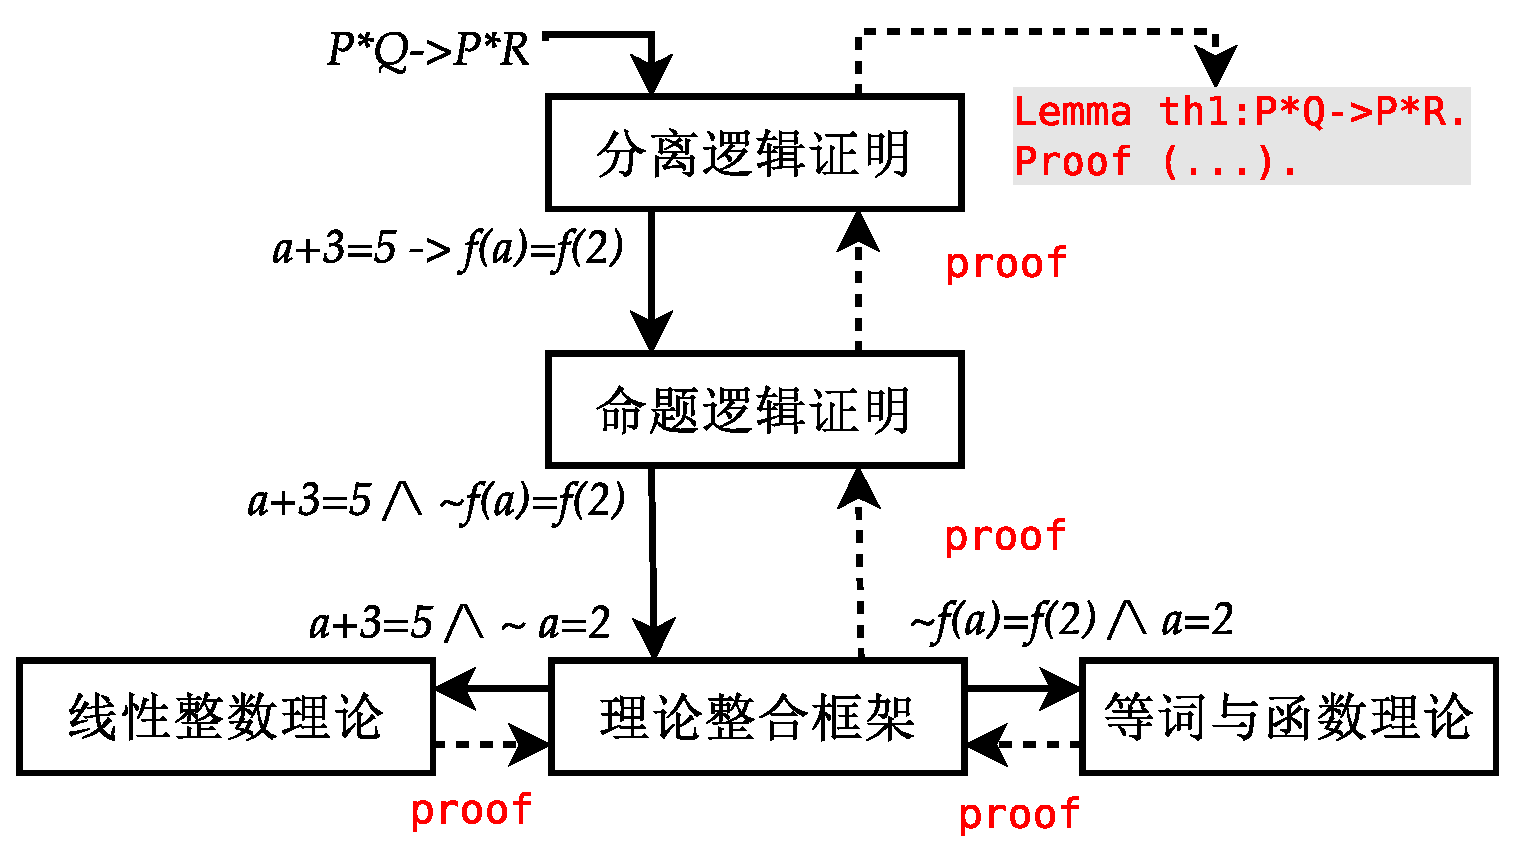
\includegraphics[width=0.8\textwidth]{stru.eps}
  \caption{证明器的结构}
  \label{struct:fig}
\end{figure}

如图\ref{struct:fig}所示,证明器逻辑上可以分成两大部分。一部分是传统的基于一阶逻辑的证明器;另一个部分是分离逻辑的证明器。

\subsection{分离逻辑的证明器所做的工作}
证明器开始运行时,接收命题语言$\Pi \land \Sigma \impl \Pi' \land \Sigma'$。

这个命题的证明可以化为求证:
\begin{eqnarray}
  \vdash & \Pi \land \Pi'' \impl \Pi' \label{struct:eq1}\\
  \vdash & \Pi \land \Sigma \impl \Sigma' \label{struct:eq2}
\end{eqnarray}

\ref{struct:eq1}式是一个纯的一阶逻辑的证明过程,因此直接将该部分命题发送到一阶逻辑的证明器求证。其中$\Pi''$是分离逻辑部分中推出的一些算术信息,如指针非空和不同堆的地址不同。

\ref{struct:eq2}式是一个带分离逻辑的证明过程。该部分将由分离逻辑的证明器使用分离逻辑中的定理将该过程分解成求证一系列纯一阶逻辑命题,并发送到一阶逻辑的证明器求证。该部分的方法在第\ref{chap:sep}章说明。

分离逻辑的证明器综合两式,得到命题的最终证明。

\subsection{一阶逻辑的证明器所做的工作}
一阶逻辑的证明器结构属于目前较先进的SMT(Satisfiability Modulo Theories)证明器结构。

对于每一个被发送到一阶逻辑的证明器的命题,首先经过命题逻辑证明模块。该模块将所有不同的公式项看作一个独立的命题变元,最终化简成为约束满足(SAT)问题,该步的具体方法在第\ref{chap:sat}章说明。

由于命题逻辑证明求解时不会关心命题公式项的具体内容,因此它在求解时会生成一系列可能否证命题的``反例''赋值。这些``反例''重新构成命题后被发送到理论整合框架。在这个框架中,命题被按照公式项分成不同的部分,送给不同的理论求解器求解。由于考察公式项的具体结构,``反例''将被一一反驳。该步具体方法在第\ref{chap:euf}、\ref{chap:lia}、\ref{chap:no}章说明。

命题逻辑证明模块综合这些反驳信息,得到一阶逻辑命题的最终证明。
 %证明器的总体设计
  \chapter{Coq证明项的构造概述}
\label{chap:proof}

\section{Coq}
\section{证明项的数据结构}
\begin{figure}[!htbp]
  \centering
  \begin{tabular}[rcl]{rcl}
    $E$ & \sep{} & Id \deli{} $\lambda(x:T).E$ \deli{} $(E E)$
  \end{tabular}
\end{figure}

\section{证明项构造的主要方法}
  %Coq证明项的构造概述
  \chapter{命题逻辑命题的证明}
\label{chap:sat}

\section{输入语言}

\section{决策过程}
\subsection{DPLL框架}
\subsection{实现}
\subsection{证明项的构造}

\section{命题的规范化}
    %命题逻辑命题的证明
  \chapter{等词与未解释函数理论命题的证明}
\label{chap:euf}

\section{输入语言}
\begin{figure}[!htbp]
  \centering
  \begin{tabular}[rcl]{rcl}
    $E$ & \sep{} & $x$ \deli{} $a$ \deli{} $f_i(E,$\ldots$,E)$ \\
    $T$ & \sep{} & $E = E$ \deli{} $E \neq E$ \\
    $\Pi$ & \sep{} & $T$ \deli{} $\Pi \land \Pi$ \\
  \end{tabular}
\end{figure}
\section{决策过程}
\subsection{一致闭包}
\subsection{实现}
\subsection{证明项的构造}
    %等词与未解释函数理论命题的证明
  \chapter{线性整数理论命题的证明}
\label{chap:lia}

\section{输入语言}
\begin{figure}[!htbp]
  \centering
  \begin{tabular}[rcl]{rcl}
    & & $C$是整数常元 \\
    & & $X$是整型变元 \\
    $T$ & \sep{} & $C$ \deli{} $X$ \deli{} $+(T, T)$ \deli{} $\cdot(C, T)$ \\
    $Y$ & \sep{} & $T = T$ \deli{} $T \neq T$ \deli{} $T \leq T$ \deli{} $T > T$ \\
    $\Pi$ & \sep{} & $T$ \deli{} $\Pi \land \Pi$ \\
  \end{tabular}
\end{figure}
本部分接收的语言是关于整数环上的线性不等式组,目标是证明不等式组的不可满足性。

\section{结构}
\section{单纯形法}
\subsection{标准型}
单纯形法是线性规划理论中的一种最优化方法。

原始的单纯形法解决的问题的标准型为:
\begin{eqnarray*}
  \max Z = c_1x_1 + c_2x_2 + \cdots + c_nx_n \\
  \begin{cases}
    a_{11}x_1 + a_{12}x_2 + \cdots + a_{1n}x_n = b_1 \\
    a_{21}x_1 + a_{22}x_2 + \cdots + a_{2n}x_n = b_2 \\
    \dots \\
    a_{m1}x_1 + a_{m2}x_2 + \cdots + a_{mn}x_n = b_m \\
    x_j \ge 0, \quad j = 1, 2, \cdots, n \\
    b_i \ge 0, \quad i = 1, 2, \cdots, m \\
  \end{cases}
\end{eqnarray*}
任意的线性规划问题经过适当变换后均可以转换为标准型。

单纯形法在求解时,首先要找到一组初始解,它满足约束条件,但未必最优。接下来,从初始解开始经过一系列迭代,最终达到最优解。如果初始解找不到,则说明问题无解。

单纯形法找初始解的特性为线性不等式组的可满足判定提供了一种天然方法。即若能找到初始解,则不等式组可满足,否则不可满足。

依据上述思路,定义本文中单纯形法解决可满足问题的标准型如下:
\begin{eqnarray*}
  \begin{cases}
    a_{11}x_1 + a_{12}x_2 + \cdots + a_{1n}x_n = s_1 \\
    a_{21}x_1 + a_{22}x_2 + \cdots + a_{2n}x_n = s_2 \\
    \dots \\
    a_{m1}x_1 + a_{m2}x_2 + \cdots + a_{mn}x_n = s_m \\
    x_j \textrm{无限制}, \quad j = 1, 2, \cdots, n \\
    s_i \le b_i, \quad i = 1, 2, \cdots, m \\
    b_i \in \mathbb{Q}, \quad i = 1, 2, \cdots, m \\
  \end{cases}
\end{eqnarray*}

上述标准型中去掉了优化函数$Z$,因为可满足求解不关心;其次将$x_j$的限制放开,减少变换负担;最后在等式右边加入了$m$个有界的\emph{松弛变量},作用也是减少通常形式到标准型的负担。

\section{规范化过程}
    %线性整数理论命题的证明
  \chapter{理论整合框架的实现}
\label{chap:no}

理论整合框架的作用是,将一个含有多种理论的命题分解成一组命题,两者的可满足性是相同的,且命题组的每一个命题只含某一个理论所能处理的符号。

\section{Nelson-Oppen框架}
Nelson-Oppen框架\cite{Nelson:1979:SCD:357073.357079}是Nelson和Oppen提出的解决理论整合的方案。它的主要步骤如下:
\begin{description}
  \item[纯化] 通过引入新变量,将混合的理论分开。

    如命题$x = 1 \land f(2) = 1 \land \lnot f(+(1,x))=1$经过纯化后,变成$x = u \land f(v) = u \land \lnot f(w)=u$和$u = 1 \land v = 2 \land w = +(1, x)$,前者属于等词与未解释函数理论,后者属于线性整数理论。
  \item[证明] 将纯化公式送往对应理论求解器求解。若某个理论返回``不可满足'',则返回``不可满足''。
  \item[等式传播] 分如下情况:

    若某理论能够推出等式$x = y$,将$x = y$加入其他理论并重启证明。

    若某个理论能够推出$x_1 = y_1 \lor \cdots \lor x_k = y_k$,则分成k种情况,依次将$x_1 = y_1, \dots, x_k = y_k$加入其他理论并证明。若某一种情况返回``可满足'',则返回可满足;否则返回``不可满足''。

    若无法推出新的等式,返回``可满足''。
\end{description}

\section{实现}
Nelson-Oppen框架实现的难点在于等式传播,而其他部分的实现都是直接的。

等式传播的主要问题是,前述的两种理论求解器都只能证实结论,却不能主动推出结论。

如对于命题$x \leq 1 \land 1 leq x \impl f(x) = f(1)$,经过否定并规范化后得到$x \leq 1 \land 1 \leq x \land \lnot f(x) = f(1)$。我们的期望是$x \leq 1 \land 1 \leq x$送给线性整数求解器得到$x=1$,然后将等式传播给未解释函数求解器,就能得到不可满足的结论。

本文试图采用\emph{推出式}的方法,即改造线性整数求解器,使之能够在某些可满足的情形下附加一组等式,提供闭合可行域中的所有取值,然后一一送给其他求解器求解。这种改造方法在一些特殊的例子下工作得很好,甚至能够解决形如$1 \leq x \land x \leq 3 \land f(1)=1 \land f(2)=2 \land f(3)=3 \impl f(x)=x$这样的``归纳型''命题。

然而,处理命题$x \leq y \land y \leq x \impl f(x) = f(y)$时却遇到困难。原因是条件$x \leq y \land y$确定的区域含有无限个点。若不传播,则命题无法证明;若传播,则会进入死循环。一种办法是让未解释函数求解器也作出提示,如由$\lnot f(x) = f(y)$猜测线性整数证明器应该证明$x=y$。这种方法目前正在继续尝试。

另外还存在\emph{穷举式}的方法,由材料\cite{Harrison:2009:HPL:1540610}给出。它会穷举所有中间结论,并一一尝试证明,因此能够解决推出式的方法。这种方法不需要对理论证明器做修改,模块性较好。这种方法相对于推出式,不能利用具体理论的特性,因此预期性能会下降。

\section{证明项的生成}
Nelson-Oppen框架涉及证明项求解的部分是命题的纯化部分。

仍以
$$x = 1 \land f(2) = 1 \land \lnot f(+(1,x))=1$$
为例说明如何生成证明项。

上述命题在纯化之后,实际证明的是
$$x = u \land f(v) = u \land \lnot f(w)=u \land u = 1 \land v = 2 \land w = +(1, x) \impl false$$

下面构造
\begin{align*}
x = 1 \land f(2) = 1 \land \lnot f(+(1,x))=1 \impl \\
x = u \land f(v) = u \land \lnot f(w)=u \land u = 1 \land v = 2 \land w = +(1, x)
\end{align*}
的证明项,然后应用$\impl$的传递特征,就能得到
$$x = 1 \land f(2) = 1 \land \lnot f(+(1,x))=1 \impl false$$
的证明项。

而证明项可由下述Coq的引理构造:
\begin{verbatim}
Lemma eq_ind : forall (A : Type) (x : A) (P : A -> Prop),
               P x -> forall y : A, x = y -> P y .
\end{verbatim}

这就完成了证明项的构造。
     %理论整合框架的实现
  \chapter{分离逻辑命题的证明}
\label{chap:sep}

\section{语言}

\section{证明方案}
    %分离逻辑命题的证明
  \chapter{总结}
\label{chap:end}

\section{论文工作总结}

\section{进一步的工作}

    %总结

%%%%%%%%%%%%%%%%%%%%%%%%%%%%%%
%% 附件部分
%%%%%%%%%%%%%%%%%%%%%%%%%%%%%%
%\backmatter

  % 参考文献
  % 使用 BibTeX
  \phantomsection
  \addcontentsline{toc}{chapter}{参考文献}
  \bibliography{tex}
  \nocite{*} % for every item


  % 附录
  \begin{appendix}
    \chapter{附录}
\label{chap:app}

附录是作为说明书(论文)的补充部分,并不是必需的。

  \end{appendix}



\end{document}
